   \documentclass{article}
\usepackage{pgfplots}
\begin{document}
\begin{figure}
\centering

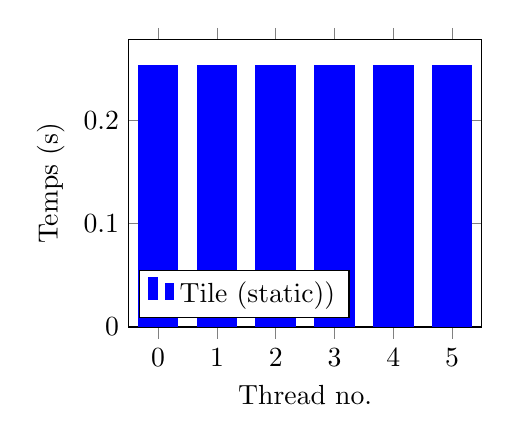
\begin{tikzpicture}
\begin{axis}[
  ybar,
  bar width=0.5cm,
  xlabel={Thread no.},
  ylabel={Temps (s)},
  ymin=0,
  legend pos=south west,
  width=0.5\textwidth,
  xtick=data
]

% Données pour le premier graphique (à gauche)
\addplot[color=blue, fill=blue] coordinates {
  (0,0.252563) (1,0.252560) (2,0.252597) (3,0.252597) (4,0.252566) (5,0.252703)
};
\addlegendentry{Tile (static))}

\end{axis}
\end{tikzpicture}
\hfill
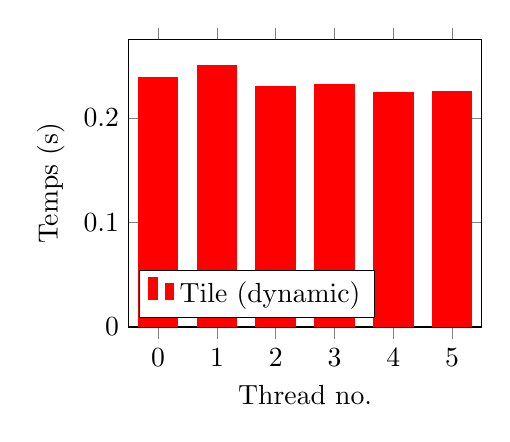
\begin{tikzpicture}
\begin{axis}[
  ybar,
  bar width=0.5cm,
  xlabel={Thread no.},
  ylabel={Temps (s)},
  ymin=0,
  legend pos=south west,
  width=0.5\textwidth,
  xtick=data
]

% Données pour le deuxième graphique (au milieu)
\addplot[color=red, fill=red] coordinates {
  (0,0.238529) (1,0.249775) (2,0.229982) (3,0.231689) (4,0.224229) (5,0.224939)
};
\addlegendentry{Tile (dynamic)}

\end{axis}
\end{tikzpicture}
\hfill
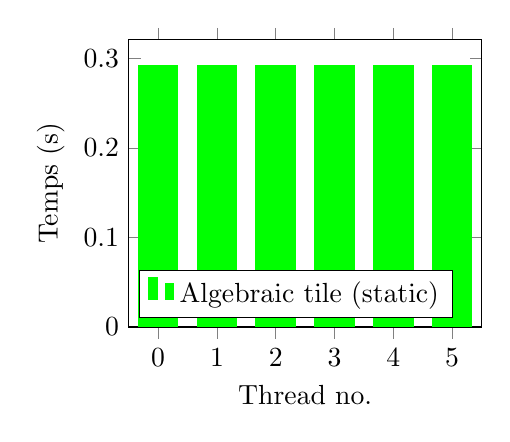
\begin{tikzpicture}
\begin{axis}[
  ybar,
  bar width=0.5cm,
  xlabel={Thread no.},
  ylabel={Temps (s)},
  ymin=0,
  legend pos=south west,
  width=0.5\textwidth,
  xtick=data
]

% Données pour le troisième graphique (à droite)
\addplot[color=green, fill=green] coordinates {
  (0,0.291574) (1,0.291568) (2,0.291572) (3,0.291571) (4,0.291568) (5,0.291573)
};
\addlegendentry{Algebraic tile (static)}

\end{axis}
\end{tikzpicture}

\caption{Temps d'exécution des threads pour le fichier gemm.c}
\label{fig:graphes}
\end{figure}

\begin{table}[htbp]
  \centering
  \caption{Statistiques pour le fichier gemm.c}
  \begin{tabular}{|c|c|c|c|}
    \hline
    Statistique & Algebraic Tile & Tile (static) & Tile (dynamic) \\ 
    \hline
    Skewness (g1) & -0.24357 & 1.42902 & 0.830889 \\ 
    Kurtosis (g2) & -1.47656 & 0.532677 & -0.562224 \\ 
    Écart type & 2.3094e-06 & 4.953e-05 & 0.00879858\\ 
    Percent Imbalance metric en \% & 0.00102891 & 0.041568 & 7.11223\\ 
    Temps moyen (s) & 0.291574 & 0.252703 & 0.249775 \\ 
    \hline
  \end{tabular}
\end{table}
\newpage

\begin{figure}
\centering

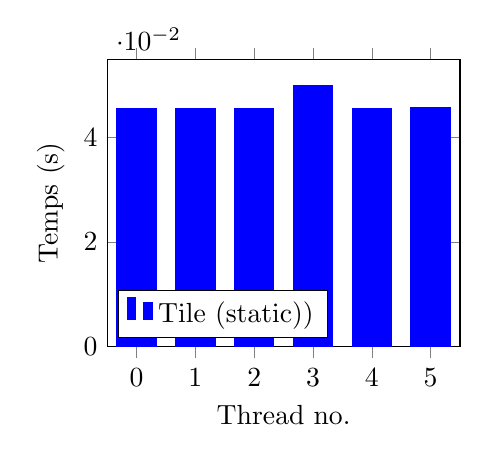
\begin{tikzpicture}
\begin{axis}[
  ybar,
  bar width=0.5cm,
  xlabel={Thread no.},
  ylabel={Temps (s)},
  ymin=0,
  legend pos=south west,
  width=0.5\textwidth,
  xtick=data
]

% Données pour le premier graphique (à gauche)
\addplot[color=blue, fill=blue] coordinates {
  (0,0.045526) (1,0.045522) (2,0.045524) (3,0.049872) (4,0.045522) (5,0.045578)
};
\addlegendentry{Tile (static))}

\end{axis}
\end{tikzpicture}
\hfill
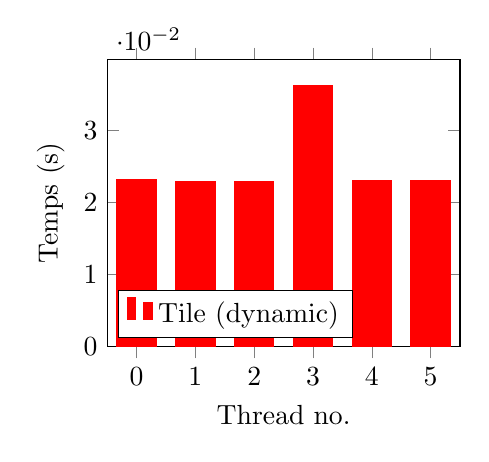
\begin{tikzpicture}
\begin{axis}[
  ybar,
  bar width=0.5cm,
  xlabel={Thread no.},
  ylabel={Temps (s)},
  ymin=0,
  legend pos=south west,
  width=0.5\textwidth,
  xtick=data
]

% Données pour le deuxième graphique (au milieu)
\addplot[color=red, fill=red] coordinates {
  (0,0.023156) (1,0.022906) (2,0.022869) (3,0.036181) (4,0.022966) (5,0.023045)
};
\addlegendentry{Tile (dynamic)}

\end{axis}
\end{tikzpicture}
\hfill
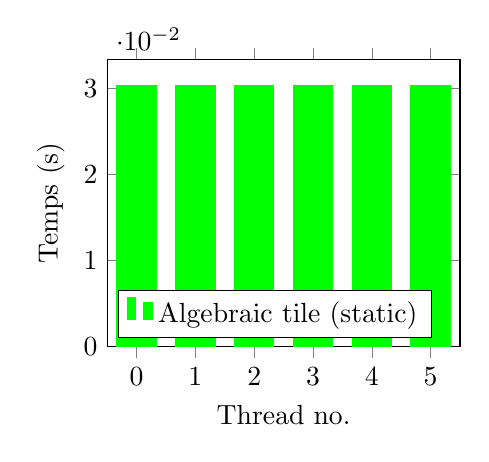
\begin{tikzpicture}
\begin{axis}[
  ybar,
  bar width=0.5cm,
  xlabel={Thread no.},
  ylabel={Temps (s)},
  ymin=0,
  legend pos=south west,
  width=0.5\textwidth,
  xtick=data
]

% Données pour le troisième graphique (à droite)
\addplot[color=green, fill=green] coordinates {
  (0,0.030312) (1,0.030315) (2,0.030313) (3,0.030311) (4,0.030311) (5,0.030357)
};
\addlegendentry{Algebraic tile (static)}

\end{axis}
\end{tikzpicture}

\caption{Temps d'exécution des threads pour le fichier gemver.c}
\label{fig:graphes}
\end{figure}

\begin{table}[htbp]
  \centering
  \caption{Statistiques pour le fichier gemver.c}
  \begin{tabular}{|c|c|c|c|}
    \hline
    Statistique & Algebraic Tile & Tile (static) & Tile (dynamic) \\ 
    \hline
    Skewness (g1) & 1.76234 & 1.78824 & 1.78739 \\ 
    Kurtosis (g2) & 1.15115 & 1.1989 & 1.19737 \\ 
    Écart type & 1.66775e-05 & 0.00161665 & 0.00491749\\ 
    Percent Imbalance metric en \% & 0.122692 & 7.81433 & 43.6484\\ 
    Temps moyen (s) & 0.030357 & 0.049872 & 0.036181 \\ 
    \hline
  \end{tabular}
\end{table}
\newpage

\begin{figure}
\centering

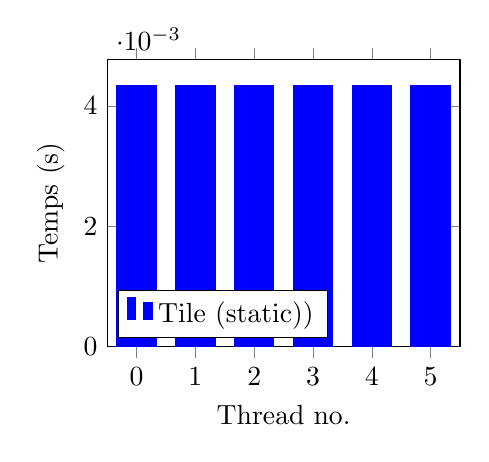
\begin{tikzpicture}
\begin{axis}[
  ybar,
  bar width=0.5cm,
  xlabel={Thread no.},
  ylabel={Temps (s)},
  ymin=0,
  legend pos=south west,
  width=0.5\textwidth,
  xtick=data
]

% Données pour le premier graphique (à gauche)
\addplot[color=blue, fill=blue] coordinates {
  (0,0.004339) (1,0.004342) (2,0.004340) (3,0.004339) (4,0.004338) (5,0.004338)
};
\addlegendentry{Tile (static))}

\end{axis}
\end{tikzpicture}
\hfill
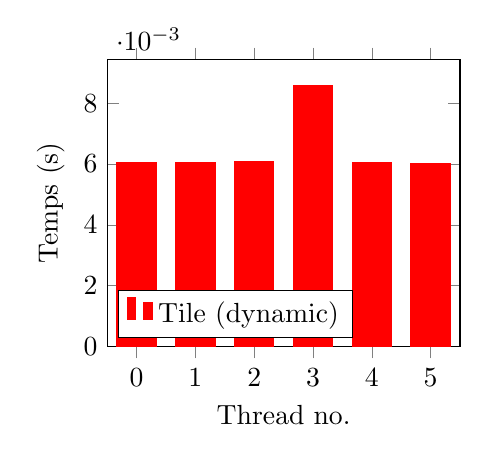
\begin{tikzpicture}
\begin{axis}[
  ybar,
  bar width=0.5cm,
  xlabel={Thread no.},
  ylabel={Temps (s)},
  ymin=0,
  legend pos=south west,
  width=0.5\textwidth,
  xtick=data
]

% Données pour le deuxième graphique (au milieu)
\addplot[color=red, fill=red] coordinates {
  (0,0.006036) (1,0.006059) (2,0.006085) (3,0.008583) (4,0.006039) (5,0.006010)
};
\addlegendentry{Tile (dynamic)}

\end{axis}
\end{tikzpicture}
\hfill
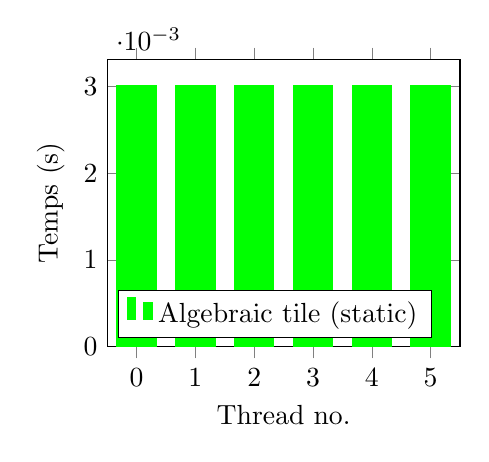
\begin{tikzpicture}
\begin{axis}[
  ybar,
  bar width=0.5cm,
  xlabel={Thread no.},
  ylabel={Temps (s)},
  ymin=0,
  legend pos=south west,
  width=0.5\textwidth,
  xtick=data
]

% Données pour le troisième graphique (à droite)
\addplot[color=green, fill=green] coordinates {
  (0,0.003006) (1,0.003010) (2,0.003005) (3,0.003006) (4,0.003005) (5,0.003005)
};
\addlegendentry{Algebraic tile (static)}

\end{axis}
\end{tikzpicture}

\caption{Temps d'exécution des threads pour le fichier gesummv.c}
\label{fig:graphes}
\end{figure}

\begin{table}[htbp]
  \centering
  \caption{Statistiques pour le fichier gesummv.c}
  \begin{tabular}{|c|c|c|c|}
    \hline
    Statistique & Algebraic Tile & Tile (static) & Tile (dynamic) \\ 
    \hline
    Skewness (g1) & 1.54511 & 0.927342 & 1.78651 \\ 
    Kurtosis (g2) & 0.746652 & -0.33218 & 1.19579 \\ 
    Écart type & 1.77169e-06 & 1.37437e-06 & 0.000945835\\ 
    Percent Imbalance metric en \% & 0.127405 & 0.0615302 & 32.6857\\ 
    Temps moyen (s) & 0.003010 & 0.004342 & 0.008583 \\ 
    \hline
  \end{tabular}
\end{table}
\newpage

\begin{figure}
\centering

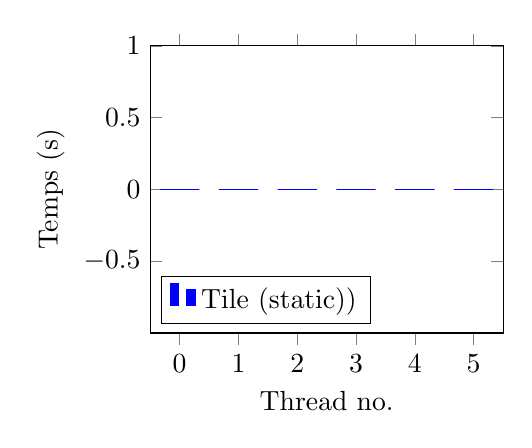
\begin{tikzpicture}
\begin{axis}[
  ybar,
  bar width=0.5cm,
  xlabel={Thread no.},
  ylabel={Temps (s)},
  ymin=0,
  legend pos=south west,
  width=0.5\textwidth,
  xtick=data
]

% Données pour le premier graphique (à gauche)
\addplot[color=blue, fill=blue] coordinates {
  (0,0.000000) (1,0.000000) (2,0.000000) (3,0.000000) (4,0.000000) (5,0.000000)
};
\addlegendentry{Tile (static))}

\end{axis}
\end{tikzpicture}
\hfill
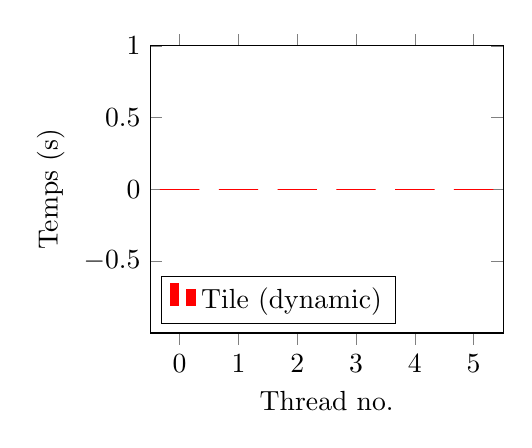
\begin{tikzpicture}
\begin{axis}[
  ybar,
  bar width=0.5cm,
  xlabel={Thread no.},
  ylabel={Temps (s)},
  ymin=0,
  legend pos=south west,
  width=0.5\textwidth,
  xtick=data
]

% Données pour le deuxième graphique (au milieu)
\addplot[color=red, fill=red] coordinates {
  (0,0.000000) (1,0.000000) (2,0.000000) (3,0.000000) (4,0.000000) (5,0.000000)
};
\addlegendentry{Tile (dynamic)}

\end{axis}
\end{tikzpicture}
\hfill
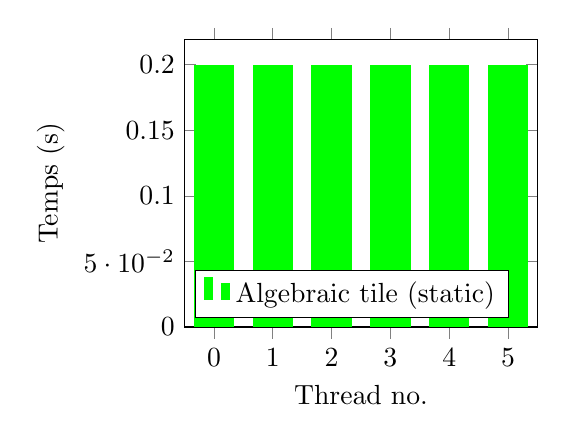
\begin{tikzpicture}
\begin{axis}[
  ybar,
  bar width=0.5cm,
  xlabel={Thread no.},
  ylabel={Temps (s)},
  ymin=0,
  legend pos=south west,
  width=0.5\textwidth,
  xtick=data
]

% Données pour le troisième graphique (à droite)
\addplot[color=green, fill=green] coordinates {
  (0,0.199015) (1,0.199010) (2,0.199048) (3,0.199048) (4,0.199015) (5,0.199015)
};
\addlegendentry{Algebraic tile (static)}

\end{axis}
\end{tikzpicture}

\caption{Temps d'exécution des threads pour le fichier symm.c}
\label{fig:graphes}
\end{figure}

\begin{table}[htbp]
  \centering
  \caption{Statistiques pour le fichier symm.c}
  \begin{tabular}{|c|c|c|c|}
    \hline
    Statistique & Algebraic Tile & Tile (static) & Tile (dynamic) \\ 
    \hline
    Skewness (g1) & 0.667777 &  &  \\ 
    Kurtosis (g2) & -1.49459 &  &  \\ 
    Écart type & 1.62421e-05 & 0 & 0\\ 
    Percent Imbalance metric en \% & 0.0115563 &  & \\ 
    Temps moyen (s) & 0.199048 & 0 & 0 \\ 
    \hline
  \end{tabular}
\end{table}
\newpage

\begin{figure}
\centering

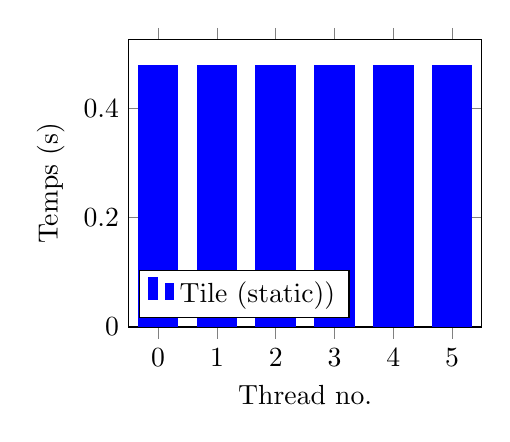
\begin{tikzpicture}
\begin{axis}[
  ybar,
  bar width=0.5cm,
  xlabel={Thread no.},
  ylabel={Temps (s)},
  ymin=0,
  legend pos=south west,
  width=0.5\textwidth,
  xtick=data
]

% Données pour le premier graphique (à gauche)
\addplot[color=blue, fill=blue] coordinates {
  (0,0.477577) (1,0.477577) (2,0.477592) (3,0.477592) (4,0.477539) (5,0.477533)
};
\addlegendentry{Tile (static))}

\end{axis}
\end{tikzpicture}
\hfill
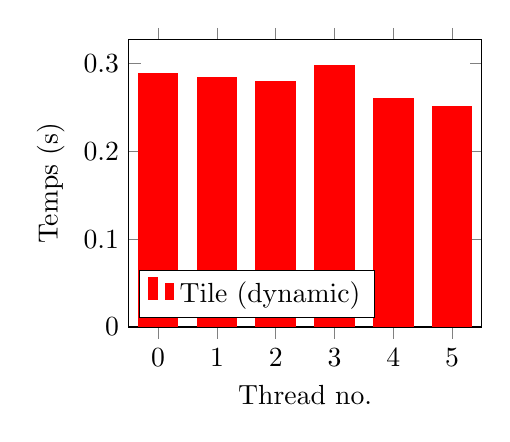
\begin{tikzpicture}
\begin{axis}[
  ybar,
  bar width=0.5cm,
  xlabel={Thread no.},
  ylabel={Temps (s)},
  ymin=0,
  legend pos=south west,
  width=0.5\textwidth,
  xtick=data
]

% Données pour le deuxième graphique (au milieu)
\addplot[color=red, fill=red] coordinates {
  (0,0.288273) (1,0.284289) (2,0.279086) (3,0.297181) (4,0.259610) (5,0.250827)
};
\addlegendentry{Tile (dynamic)}

\end{axis}
\end{tikzpicture}
\hfill
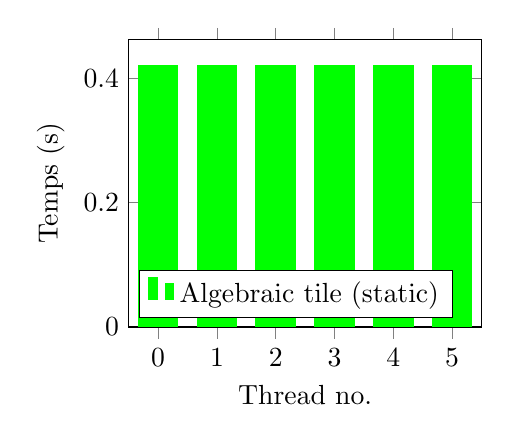
\begin{tikzpicture}
\begin{axis}[
  ybar,
  bar width=0.5cm,
  xlabel={Thread no.},
  ylabel={Temps (s)},
  ymin=0,
  legend pos=south west,
  width=0.5\textwidth,
  xtick=data
]

% Données pour le troisième graphique (à droite)
\addplot[color=green, fill=green] coordinates {
  (0,0.420013) (1,0.420009) (2,0.420072) (3,0.420072) (4,0.420058) (5,0.420058)
};
\addlegendentry{Algebraic tile (static)}

\end{axis}
\end{tikzpicture}

\caption{Temps d'exécution des threads pour le fichier syr2k.c}
\label{fig:graphes}
\end{figure}

\begin{table}[htbp]
  \centering
  \caption{Statistiques pour le fichier syr2k.c}
  \begin{tabular}{|c|c|c|c|}
    \hline
    Statistique & Algebraic Tile & Tile (static) & Tile (dynamic) \\ 
    \hline
    Skewness (g1) & -0.563936 & -0.517929 & -0.429139 \\ 
    Kurtosis (g2) & -1.48356 & -1.45653 & -1.25652 \\ 
    Écart type & 2.61151e-05 & 2.37323e-05 & 0.0162174\\ 
    Percent Imbalance metric en \% & 0.00595171 & 0.00502546 & 7.46247\\ 
    Temps moyen (s) & 0.420072 & 0.477592 & 0.297181 \\ 
    \hline
  \end{tabular}
\end{table}
\newpage

\begin{figure}
\centering

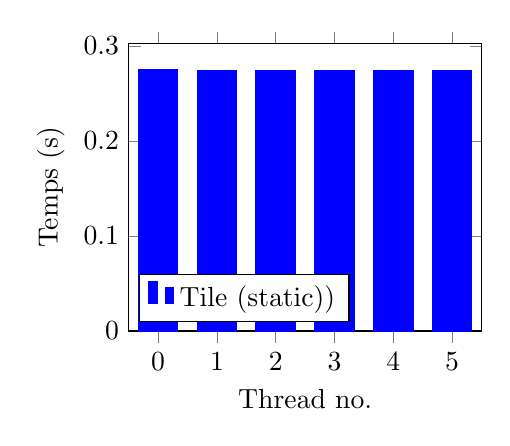
\begin{tikzpicture}
\begin{axis}[
  ybar,
  bar width=0.5cm,
  xlabel={Thread no.},
  ylabel={Temps (s)},
  ymin=0,
  legend pos=south west,
  width=0.5\textwidth,
  xtick=data
]

% Données pour le premier graphique (à gauche)
\addplot[color=blue, fill=blue] coordinates {
  (0,0.274634) (1,0.273919) (2,0.273919) (3,0.274329) (4,0.274012) (5,0.273921)
};
\addlegendentry{Tile (static))}

\end{axis}
\end{tikzpicture}
\hfill
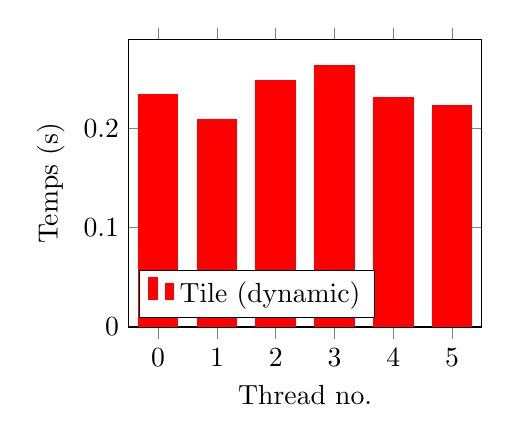
\begin{tikzpicture}
\begin{axis}[
  ybar,
  bar width=0.5cm,
  xlabel={Thread no.},
  ylabel={Temps (s)},
  ymin=0,
  legend pos=south west,
  width=0.5\textwidth,
  xtick=data
]

% Données pour le deuxième graphique (au milieu)
\addplot[color=red, fill=red] coordinates {
  (0,0.233454) (1,0.208227) (2,0.248114) (3,0.262688) (4,0.231046) (5,0.223211)
};
\addlegendentry{Tile (dynamic)}

\end{axis}
\end{tikzpicture}
\hfill
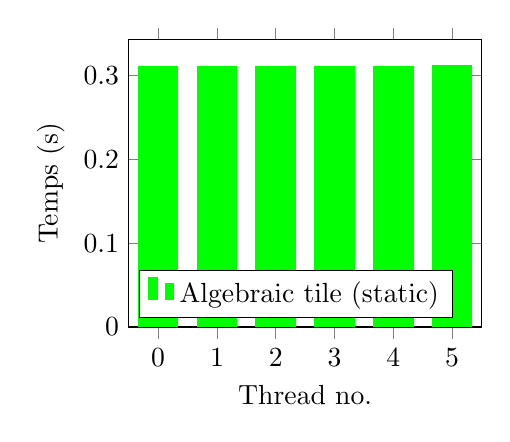
\begin{tikzpicture}
\begin{axis}[
  ybar,
  bar width=0.5cm,
  xlabel={Thread no.},
  ylabel={Temps (s)},
  ymin=0,
  legend pos=south west,
  width=0.5\textwidth,
  xtick=data
]

% Données pour le troisième graphique (à droite)
\addplot[color=green, fill=green] coordinates {
  (0,0.311300) (1,0.311294) (2,0.311303) (3,0.311301) (4,0.311295) (5,0.311613)
};
\addlegendentry{Algebraic tile (static)}

\end{axis}
\end{tikzpicture}

\caption{Temps d'exécution des threads pour le fichier syrk.c}
\label{fig:graphes}
\end{figure}

\begin{table}[htbp]
  \centering
  \caption{Statistiques pour le fichier syrk.c}
  \begin{tabular}{|c|c|c|c|}
    \hline
    Statistique & Algebraic Tile & Tile (static) & Tile (dynamic) \\ 
    \hline
    Skewness (g1) & 1.78586 & 0.977741 & 0.176109 \\ 
    Kurtosis (g2) & 1.19467 & -0.656857 & -0.877951 \\ 
    Écart type & 0.000117213 & 0.000270774 & 0.0173716\\ 
    Percent Imbalance metric en \% & 0.0841494 & 0.186778 & 12.041\\ 
    Temps moyen (s) & 0.311613 & 0.274634 & 0.262688 \\ 
    \hline
  \end{tabular}
\end{table}
\newpage

\begin{figure}
\centering

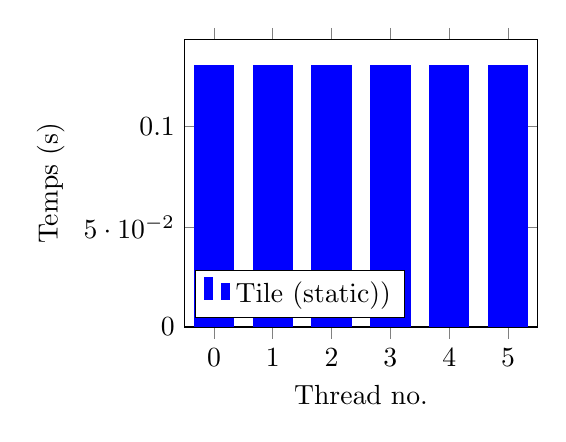
\begin{tikzpicture}
\begin{axis}[
  ybar,
  bar width=0.5cm,
  xlabel={Thread no.},
  ylabel={Temps (s)},
  ymin=0,
  legend pos=south west,
  width=0.5\textwidth,
  xtick=data
]

% Données pour le premier graphique (à gauche)
\addplot[color=blue, fill=blue] coordinates {
  (0,0.130354) (1,0.130362) (2,0.130401) (3,0.130401) (4,0.130364) (5,0.130364)
};
\addlegendentry{Tile (static))}

\end{axis}
\end{tikzpicture}
\hfill
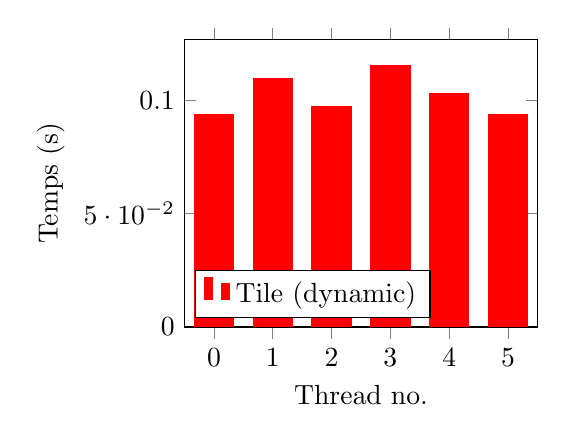
\begin{tikzpicture}
\begin{axis}[
  ybar,
  bar width=0.5cm,
  xlabel={Thread no.},
  ylabel={Temps (s)},
  ymin=0,
  legend pos=south west,
  width=0.5\textwidth,
  xtick=data
]

% Données pour le deuxième graphique (au milieu)
\addplot[color=red, fill=red] coordinates {
  (0,0.093454) (1,0.109617) (2,0.097217) (3,0.115109) (4,0.103102) (5,0.093816)
};
\addlegendentry{Tile (dynamic)}

\end{axis}
\end{tikzpicture}
\hfill
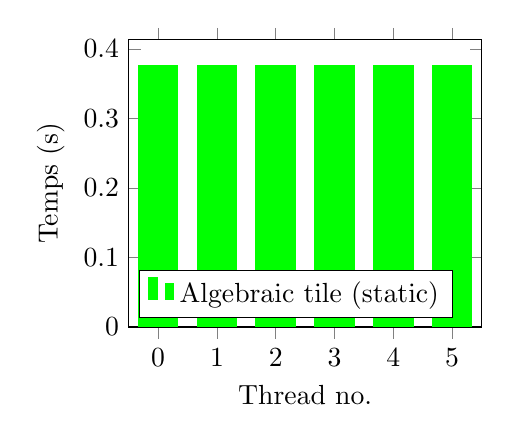
\begin{tikzpicture}
\begin{axis}[
  ybar,
  bar width=0.5cm,
  xlabel={Thread no.},
  ylabel={Temps (s)},
  ymin=0,
  legend pos=south west,
  width=0.5\textwidth,
  xtick=data
]

% Données pour le troisième graphique (à droite)
\addplot[color=green, fill=green] coordinates {
  (0,0.375744) (1,0.375738) (2,0.375744) (3,0.375740) (4,0.375776) (5,0.375776)
};
\addlegendentry{Algebraic tile (static)}

\end{axis}
\end{tikzpicture}

\caption{Temps d'exécution des threads pour le fichier trmm.c}
\label{fig:graphes}
\end{figure}

\begin{table}[htbp]
  \centering
  \caption{Statistiques pour le fichier trmm.c}
  \begin{tabular}{|c|c|c|c|}
    \hline
    Statistique & Algebraic Tile & Tile (static) & Tile (dynamic) \\ 
    \hline
    Skewness (g1) & 0.653682 & 0.603258 & 0.423606 \\ 
    Kurtosis (g2) & -1.49829 & -1.47924 & -1.33948 \\ 
    Écart type & 1.64012e-05 & 1.91543e-05 & 0.008103\\ 
    Percent Imbalance metric en \% & 0.00612104 & 0.0207097 & 12.7934\\ 
    Temps moyen (s) & 0.375776 & 0.130401 & 0.115109 \\ 
    \hline
  \end{tabular}
\end{table}
\newpage

\begin{figure}
\centering

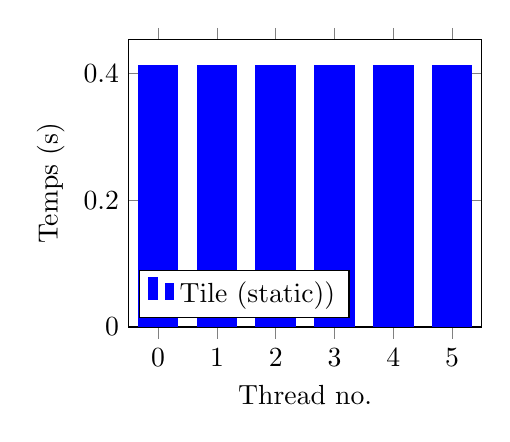
\begin{tikzpicture}
\begin{axis}[
  ybar,
  bar width=0.5cm,
  xlabel={Thread no.},
  ylabel={Temps (s)},
  ymin=0,
  legend pos=south west,
  width=0.5\textwidth,
  xtick=data
]

% Données pour le premier graphique (à gauche)
\addplot[color=blue, fill=blue] coordinates {
  (0,0.412175) (1,0.412173) (2,0.412174) (3,0.412174) (4,0.412169) (5,0.412166)
};
\addlegendentry{Tile (static))}

\end{axis}
\end{tikzpicture}
\hfill
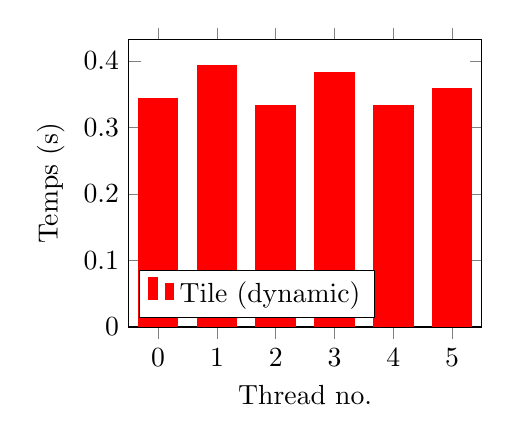
\begin{tikzpicture}
\begin{axis}[
  ybar,
  bar width=0.5cm,
  xlabel={Thread no.},
  ylabel={Temps (s)},
  ymin=0,
  legend pos=south west,
  width=0.5\textwidth,
  xtick=data
]

% Données pour le deuxième graphique (au milieu)
\addplot[color=red, fill=red] coordinates {
  (0,0.342942) (1,0.392371) (2,0.332267) (3,0.382248) (4,0.332529) (5,0.358857)
};
\addlegendentry{Tile (dynamic)}

\end{axis}
\end{tikzpicture}
\hfill
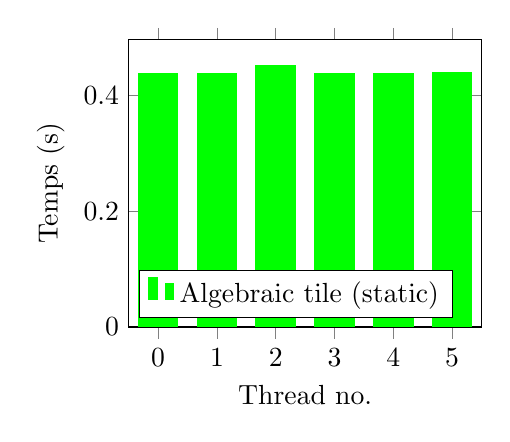
\begin{tikzpicture}
\begin{axis}[
  ybar,
  bar width=0.5cm,
  xlabel={Thread no.},
  ylabel={Temps (s)},
  ymin=0,
  legend pos=south west,
  width=0.5\textwidth,
  xtick=data
]

% Données pour le troisième graphique (à droite)
\addplot[color=green, fill=green] coordinates {
  (0,0.438351) (1,0.438322) (2,0.451074) (3,0.438345) (4,0.438355) (5,0.439227)
};
\addlegendentry{Algebraic tile (static)}

\end{axis}
\end{tikzpicture}

\caption{Temps d'exécution des threads pour le fichier 2mm.c}
\label{fig:graphes}
\end{figure}

\begin{table}[htbp]
  \centering
  \caption{Statistiques pour le fichier 2mm.c}
  \begin{tabular}{|c|c|c|c|}
    \hline
    Statistique & Algebraic Tile & Tile (static) & Tile (dynamic) \\ 
    \hline
    Skewness (g1) & 1.77034 & -0.824042 & 0.37585 \\ 
    Kurtosis (g2) & 1.16507 & -0.919742 & -1.48031 \\ 
    Écart type & 0.00468973 & 3.23608e-06 & 0.0234524\\ 
    Percent Imbalance metric en \% & 2.37442 & 0.000727851 & 9.94819\\ 
    Temps moyen (s) & 0.451074 & 0.412175 & 0.392371 \\ 
    \hline
  \end{tabular}
\end{table}
\newpage

\begin{figure}
\centering

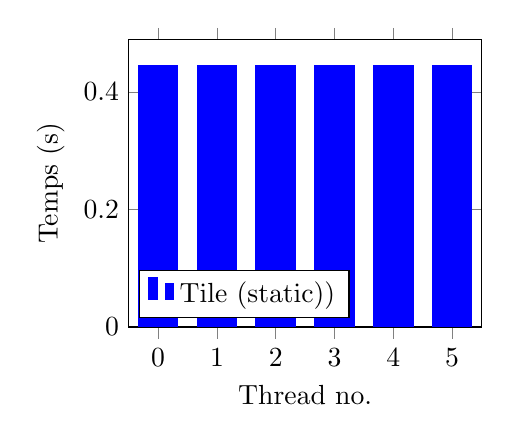
\begin{tikzpicture}
\begin{axis}[
  ybar,
  bar width=0.5cm,
  xlabel={Thread no.},
  ylabel={Temps (s)},
  ymin=0,
  legend pos=south west,
  width=0.5\textwidth,
  xtick=data
]

% Données pour le premier graphique (à gauche)
\addplot[color=blue, fill=blue] coordinates {
  (0,0.444354) (1,0.444359) (2,0.444424) (3,0.444422) (4,0.444356) (5,0.444351)
};
\addlegendentry{Tile (static))}

\end{axis}
\end{tikzpicture}
\hfill
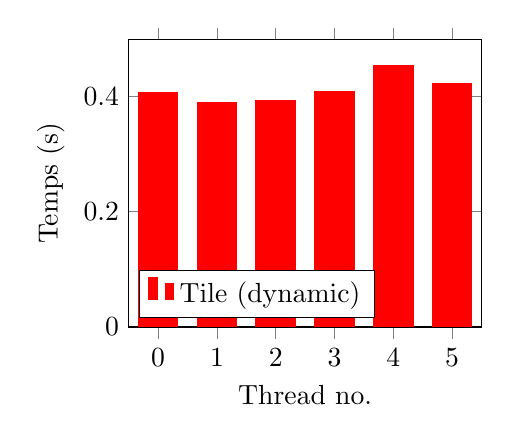
\begin{tikzpicture}
\begin{axis}[
  ybar,
  bar width=0.5cm,
  xlabel={Thread no.},
  ylabel={Temps (s)},
  ymin=0,
  legend pos=south west,
  width=0.5\textwidth,
  xtick=data
]

% Données pour le deuxième graphique (au milieu)
\addplot[color=red, fill=red] coordinates {
  (0,0.407157) (1,0.388658) (2,0.391792) (3,0.408416) (4,0.452618) (5,0.422689)
};
\addlegendentry{Tile (dynamic)}

\end{axis}
\end{tikzpicture}
\hfill
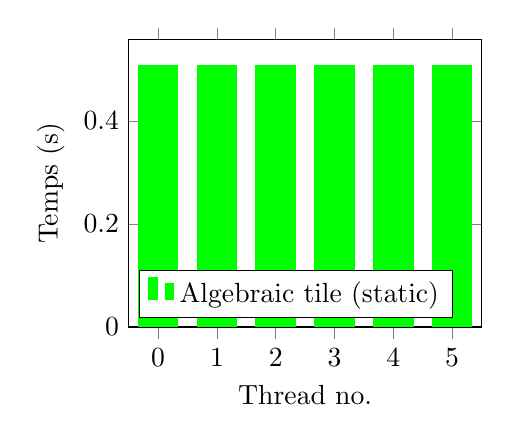
\begin{tikzpicture}
\begin{axis}[
  ybar,
  bar width=0.5cm,
  xlabel={Thread no.},
  ylabel={Temps (s)},
  ymin=0,
  legend pos=south west,
  width=0.5\textwidth,
  xtick=data
]

% Données pour le troisième graphique (à droite)
\addplot[color=green, fill=green] coordinates {
  (0,0.506787) (1,0.506810) (2,0.506860) (3,0.506856) (4,0.506928) (5,0.506928)
};
\addlegendentry{Algebraic tile (static)}

\end{axis}
\end{tikzpicture}

\caption{Temps d'exécution des threads pour le fichier 3mm.c}
\label{fig:graphes}
\end{figure}

\begin{table}[htbp]
  \centering
  \caption{Statistiques pour le fichier 3mm.c}
  \begin{tabular}{|c|c|c|c|}
    \hline
    Statistique & Algebraic Tile & Tile (static) & Tile (dynamic) \\ 
    \hline
    Skewness (g1) & 0.0415967 & 0.690726 & 0.814189 \\ 
    Kurtosis (g2) & -1.41719 & -1.49708 & -0.451371 \\ 
    Écart type & 5.33534e-05 & 3.2149e-05 & 0.0214224\\ 
    Percent Imbalance metric en \% & 0.0132186 & 0.0103515 & 9.88861\\ 
    Temps moyen (s) & 0.506928 & 0.444424 & 0.452618 \\ 
    \hline
  \end{tabular}
\end{table}
\newpage

\begin{figure}
\centering

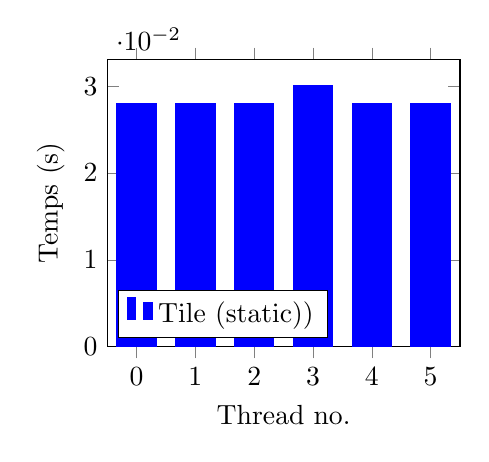
\begin{tikzpicture}
\begin{axis}[
  ybar,
  bar width=0.5cm,
  xlabel={Thread no.},
  ylabel={Temps (s)},
  ymin=0,
  legend pos=south west,
  width=0.5\textwidth,
  xtick=data
]

% Données pour le premier graphique (à gauche)
\addplot[color=blue, fill=blue] coordinates {
  (0,0.028002) (1,0.028002) (2,0.028002) (3,0.030094) (4,0.028003) (5,0.028003)
};
\addlegendentry{Tile (static))}

\end{axis}
\end{tikzpicture}
\hfill
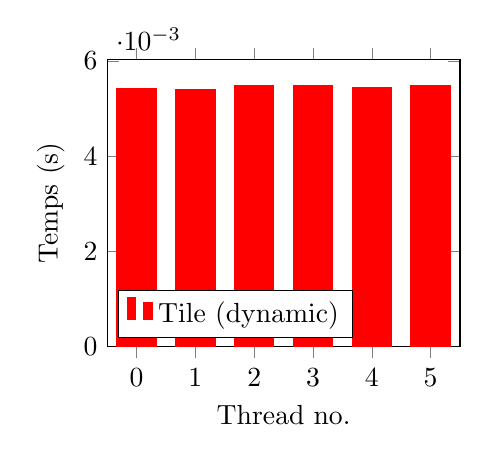
\begin{tikzpicture}
\begin{axis}[
  ybar,
  bar width=0.5cm,
  xlabel={Thread no.},
  ylabel={Temps (s)},
  ymin=0,
  legend pos=south west,
  width=0.5\textwidth,
  xtick=data
]

% Données pour le deuxième graphique (au milieu)
\addplot[color=red, fill=red] coordinates {
  (0,0.005428) (1,0.005387) (2,0.005483) (3,0.005471) (4,0.005447) (5,0.005472)
};
\addlegendentry{Tile (dynamic)}

\end{axis}
\end{tikzpicture}
\hfill
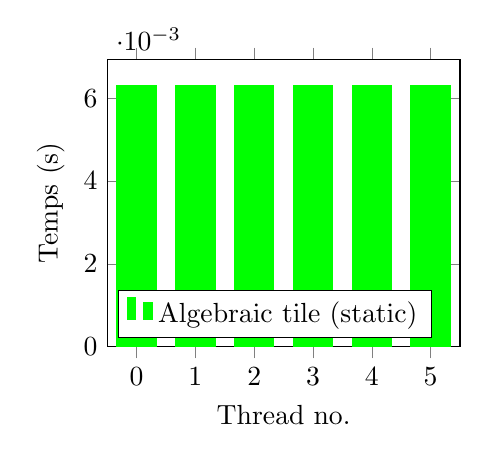
\begin{tikzpicture}
\begin{axis}[
  ybar,
  bar width=0.5cm,
  xlabel={Thread no.},
  ylabel={Temps (s)},
  ymin=0,
  legend pos=south west,
  width=0.5\textwidth,
  xtick=data
]

% Données pour le troisième graphique (à droite)
\addplot[color=green, fill=green] coordinates {
  (0,0.006305) (1,0.006308) (2,0.006307) (3,0.006305) (4,0.006305) (5,0.006305)
};
\addlegendentry{Algebraic tile (static)}

\end{axis}
\end{tikzpicture}

\caption{Temps d'exécution des threads pour le fichier atax.c}
\label{fig:graphes}
\end{figure}

\begin{table}[htbp]
  \centering
  \caption{Statistiques pour le fichier atax.c}
  \begin{tabular}{|c|c|c|c|}
    \hline
    Statistique & Algebraic Tile & Tile (static) & Tile (dynamic) \\ 
    \hline
    Skewness (g1) & 0.881181 & 1.78885 & -0.785137 \\ 
    Kurtosis (g2) & -1.0146 & 1.2 & -0.676857 \\ 
    Écart type & 1.21335e-06 & 0.000779493 & 3.27923e-05\\ 
    Percent Imbalance metric en \% & 0.0344126 & 6.14793 & 0.642438\\ 
    Temps moyen (s) & 0.006308 & 0.030094 & 0.005483 \\ 
    \hline
  \end{tabular}
\end{table}
\newpage

\begin{figure}
\centering

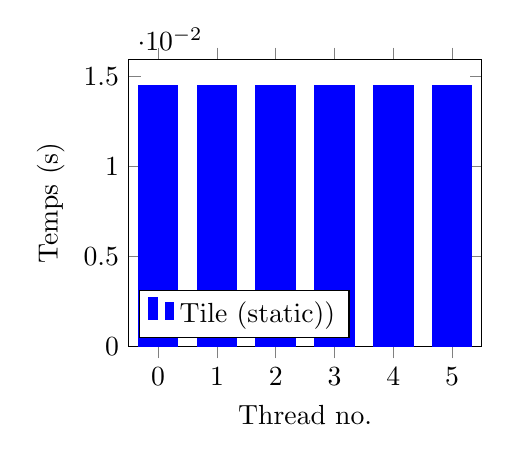
\begin{tikzpicture}
\begin{axis}[
  ybar,
  bar width=0.5cm,
  xlabel={Thread no.},
  ylabel={Temps (s)},
  ymin=0,
  legend pos=south west,
  width=0.5\textwidth,
  xtick=data
]

% Données pour le premier graphique (à gauche)
\addplot[color=blue, fill=blue] coordinates {
  (0,0.014488) (1,0.014490) (2,0.014499) (3,0.014489) (4,0.014491) (5,0.014488)
};
\addlegendentry{Tile (static))}

\end{axis}
\end{tikzpicture}
\hfill
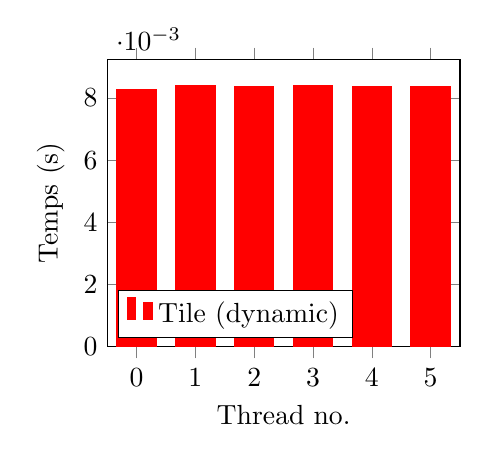
\begin{tikzpicture}
\begin{axis}[
  ybar,
  bar width=0.5cm,
  xlabel={Thread no.},
  ylabel={Temps (s)},
  ymin=0,
  legend pos=south west,
  width=0.5\textwidth,
  xtick=data
]

% Données pour le deuxième graphique (au milieu)
\addplot[color=red, fill=red] coordinates {
  (0,0.008281) (1,0.008401) (2,0.008362) (3,0.008392) (4,0.008365) (5,0.008381)
};
\addlegendentry{Tile (dynamic)}

\end{axis}
\end{tikzpicture}
\hfill
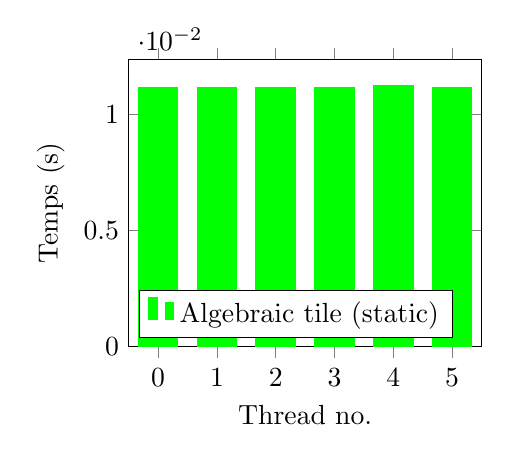
\begin{tikzpicture}
\begin{axis}[
  ybar,
  bar width=0.5cm,
  xlabel={Thread no.},
  ylabel={Temps (s)},
  ymin=0,
  legend pos=south west,
  width=0.5\textwidth,
  xtick=data
]

% Données pour le troisième graphique (à droite)
\addplot[color=green, fill=green] coordinates {
  (0,0.011164) (1,0.011180) (2,0.011166) (3,0.011166) (4,0.011251) (5,0.011164)
};
\addlegendentry{Algebraic tile (static)}

\end{axis}
\end{tikzpicture}

\caption{Temps d'exécution des threads pour le fichier bicg.c}
\label{fig:graphes}
\end{figure}

\begin{table}[htbp]
  \centering
  \caption{Statistiques pour le fichier bicg.c}
  \begin{tabular}{|c|c|c|c|}
    \hline
    Statistique & Algebraic Tile & Tile (static) & Tile (dynamic) \\ 
    \hline
    Skewness (g1) & 1.67367 & 1.49074 & -1.31695 \\ 
    Kurtosis (g2) & 0.967948 & 0.651567 & 0.399569 \\ 
    Écart type & 3.14241e-05 & 3.80424e-06 & 3.94448e-05\\ 
    Percent Imbalance metric en \% & 0.618863 & 0.0565876 & 0.446335\\ 
    Temps moyen (s) & 0.011251 & 0.014499 & 0.008401 \\ 
    \hline
  \end{tabular}
\end{table}
\newpage

\begin{figure}
\centering

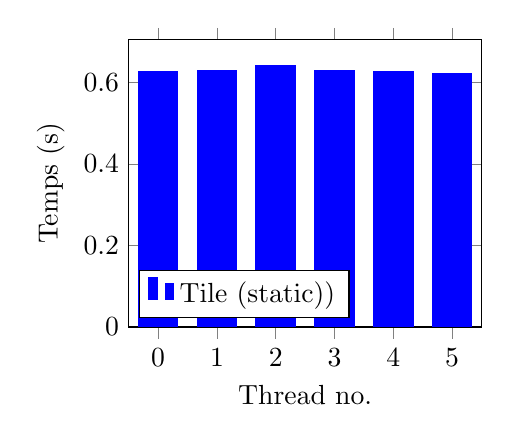
\begin{tikzpicture}
\begin{axis}[
  ybar,
  bar width=0.5cm,
  xlabel={Thread no.},
  ylabel={Temps (s)},
  ymin=0,
  legend pos=south west,
  width=0.5\textwidth,
  xtick=data
]

% Données pour le premier graphique (à gauche)
\addplot[color=blue, fill=blue] coordinates {
  (0,0.625581) (1,0.629300) (2,0.640701) (3,0.629602) (4,0.626926) (5,0.622514)
};
\addlegendentry{Tile (static))}

\end{axis}
\end{tikzpicture}
\hfill
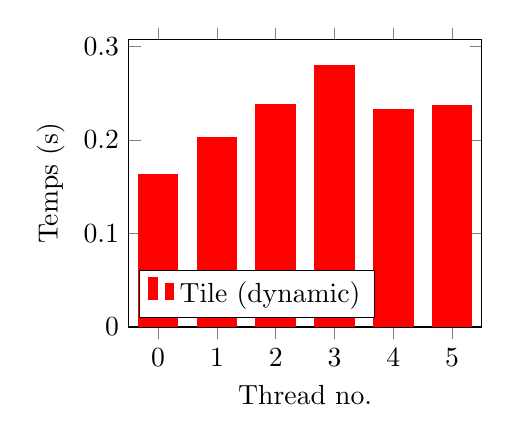
\begin{tikzpicture}
\begin{axis}[
  ybar,
  bar width=0.5cm,
  xlabel={Thread no.},
  ylabel={Temps (s)},
  ymin=0,
  legend pos=south west,
  width=0.5\textwidth,
  xtick=data
]

% Données pour le deuxième graphique (au milieu)
\addplot[color=red, fill=red] coordinates {
  (0,0.162876) (1,0.202676) (2,0.237129) (3,0.278977) (4,0.232661) (5,0.236083)
};
\addlegendentry{Tile (dynamic)}

\end{axis}
\end{tikzpicture}
\hfill
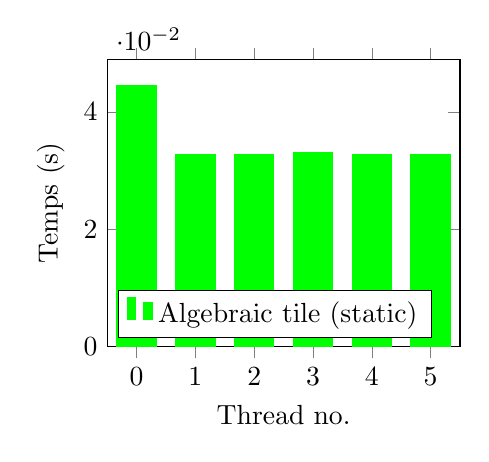
\begin{tikzpicture}
\begin{axis}[
  ybar,
  bar width=0.5cm,
  xlabel={Thread no.},
  ylabel={Temps (s)},
  ymin=0,
  legend pos=south west,
  width=0.5\textwidth,
  xtick=data
]

% Données pour le troisième graphique (à droite)
\addplot[color=green, fill=green] coordinates {
  (0,0.044482) (1,0.032736) (2,0.032738) (3,0.033025) (4,0.032735) (5,0.032733)
};
\addlegendentry{Algebraic tile (static)}

\end{axis}
\end{tikzpicture}

\caption{Temps d'exécution des threads pour le fichier doitgen.c}
\label{fig:graphes}
\end{figure}

\begin{table}[htbp]
  \centering
  \caption{Statistiques pour le fichier doitgen.c}
  \begin{tabular}{|c|c|c|c|}
    \hline
    Statistique & Algebraic Tile & Tile (static) & Tile (dynamic) \\ 
    \hline
    Skewness (g1) & 1.78651 & 1.09403 & -0.338494 \\ 
    Kurtosis (g2) & 1.19572 & 0.16782 & -0.538389 \\ 
    Écart type & 0.00435737 & 0.00570614 & 0.03559\\ 
    Percent Imbalance metric en \% & 28.0371 & 1.84342 & 23.9529\\ 
    Temps moyen (s) & 0.044482 & 0.640701 & 0.278977 \\ 
    \hline
  \end{tabular}
\end{table}
\newpage

\begin{figure}
\centering

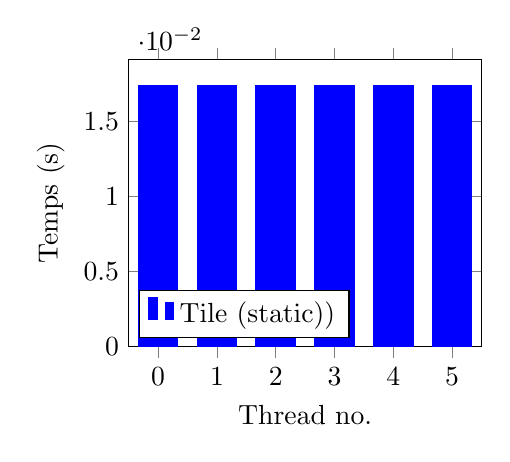
\begin{tikzpicture}
\begin{axis}[
  ybar,
  bar width=0.5cm,
  xlabel={Thread no.},
  ylabel={Temps (s)},
  ymin=0,
  legend pos=south west,
  width=0.5\textwidth,
  xtick=data
]

% Données pour le premier graphique (à gauche)
\addplot[color=blue, fill=blue] coordinates {
  (0,0.017389) (1,0.017391) (2,0.017389) (3,0.017389) (4,0.017389) (5,0.017389)
};
\addlegendentry{Tile (static))}

\end{axis}
\end{tikzpicture}
\hfill
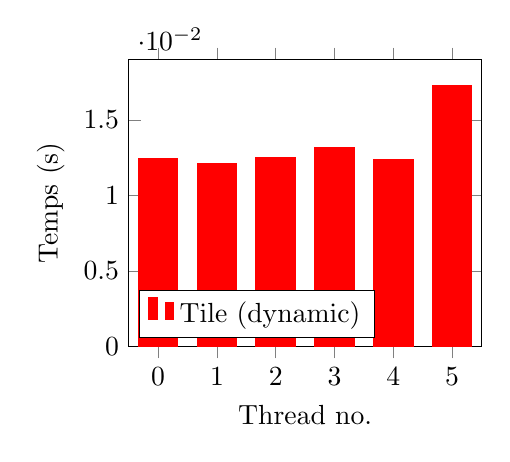
\begin{tikzpicture}
\begin{axis}[
  ybar,
  bar width=0.5cm,
  xlabel={Thread no.},
  ylabel={Temps (s)},
  ymin=0,
  legend pos=south west,
  width=0.5\textwidth,
  xtick=data
]

% Données pour le deuxième graphique (au milieu)
\addplot[color=red, fill=red] coordinates {
  (0,0.012443) (1,0.012129) (2,0.012532) (3,0.013161) (4,0.012371) (5,0.017272)
};
\addlegendentry{Tile (dynamic)}

\end{axis}
\end{tikzpicture}
\hfill
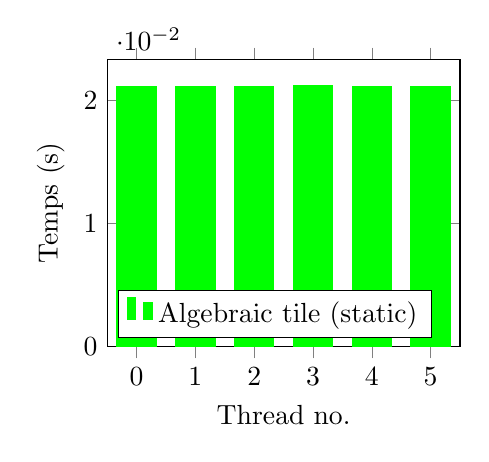
\begin{tikzpicture}
\begin{axis}[
  ybar,
  bar width=0.5cm,
  xlabel={Thread no.},
  ylabel={Temps (s)},
  ymin=0,
  legend pos=south west,
  width=0.5\textwidth,
  xtick=data
]

% Données pour le troisième graphique (à droite)
\addplot[color=green, fill=green] coordinates {
  (0,0.021115) (1,0.021115) (2,0.021121) (3,0.021206) (4,0.021115) (5,0.021115)
};
\addlegendentry{Algebraic tile (static)}

\end{axis}
\end{tikzpicture}

\caption{Temps d'exécution des threads pour le fichier mvt.c}
\label{fig:graphes}
\end{figure}

\begin{table}[htbp]
  \centering
  \caption{Statistiques pour le fichier mvt.c}
  \begin{tabular}{|c|c|c|c|}
    \hline
    Statistique & Algebraic Tile & Tile (static) & Tile (dynamic) \\ 
    \hline
    Skewness (g1) & 1.77216 & 1.78885 & 1.67242 \\ 
    Kurtosis (g2) & 1.16858 & 1.2 & 0.976159 \\ 
    Écart type & 3.35381e-05 & 7.45356e-07 & 0.00179595\\ 
    Percent Imbalance metric en \% & 0.353979 & 0.00977613 & 29.6891\\ 
    Temps moyen (s) & 0.021206 & 0.017391 & 0.017272 \\ 
    \hline
  \end{tabular}
\end{table}
\newpage

\begin{figure}
\centering

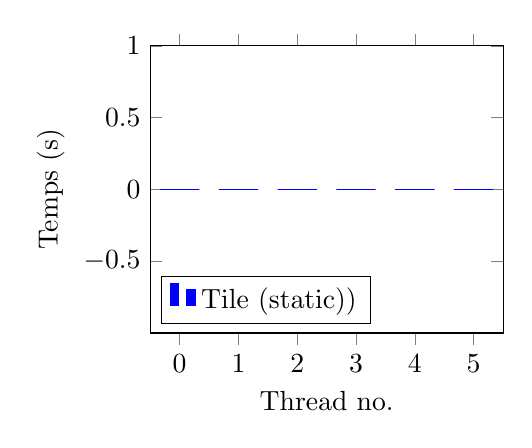
\begin{tikzpicture}
\begin{axis}[
  ybar,
  bar width=0.5cm,
  xlabel={Thread no.},
  ylabel={Temps (s)},
  ymin=0,
  legend pos=south west,
  width=0.5\textwidth,
  xtick=data
]

% Données pour le premier graphique (à gauche)
\addplot[color=blue, fill=blue] coordinates {
  (0,0.000000) (1,0.000000) (2,0.000000) (3,0.000000) (4,0.000000) (5,0.000000)
};
\addlegendentry{Tile (static))}

\end{axis}
\end{tikzpicture}
\hfill
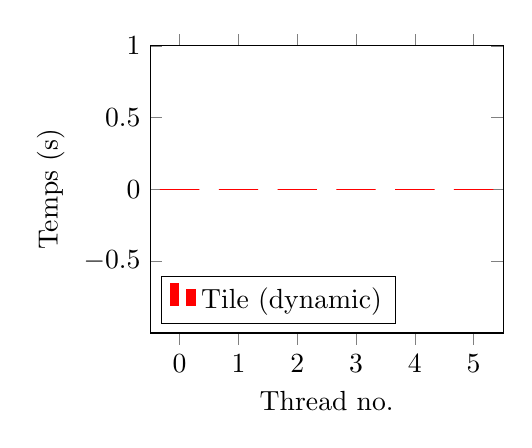
\begin{tikzpicture}
\begin{axis}[
  ybar,
  bar width=0.5cm,
  xlabel={Thread no.},
  ylabel={Temps (s)},
  ymin=0,
  legend pos=south west,
  width=0.5\textwidth,
  xtick=data
]

% Données pour le deuxième graphique (au milieu)
\addplot[color=red, fill=red] coordinates {
  (0,0.000000) (1,0.000000) (2,0.000000) (3,0.000000) (4,0.000000) (5,0.000000)
};
\addlegendentry{Tile (dynamic)}

\end{axis}
\end{tikzpicture}
\hfill
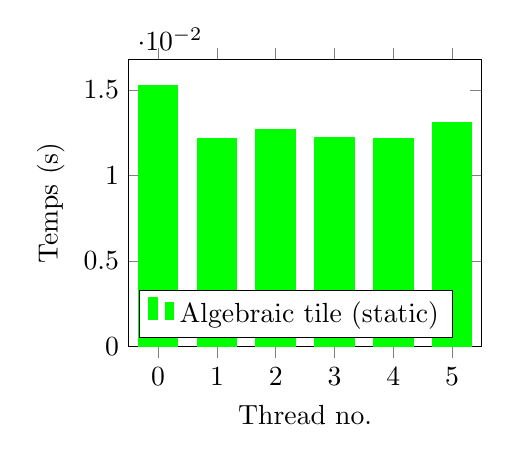
\begin{tikzpicture}
\begin{axis}[
  ybar,
  bar width=0.5cm,
  xlabel={Thread no.},
  ylabel={Temps (s)},
  ymin=0,
  legend pos=south west,
  width=0.5\textwidth,
  xtick=data
]

% Données pour le troisième graphique (à droite)
\addplot[color=green, fill=green] coordinates {
  (0,0.015259) (1,0.012177) (2,0.012691) (3,0.012200) (4,0.012178) (5,0.013086)
};
\addlegendentry{Algebraic tile (static)}

\end{axis}
\end{tikzpicture}

\caption{Temps d'exécution des threads pour le fichier durbin.c}
\label{fig:graphes}
\end{figure}

\begin{table}[htbp]
  \centering
  \caption{Statistiques pour le fichier durbin.c}
  \begin{tabular}{|c|c|c|c|}
    \hline
    Statistique & Algebraic Tile & Tile (static) & Tile (dynamic) \\ 
    \hline
    Skewness (g1) & 1.4468 &  &  \\ 
    Kurtosis (g2) & 0.531566 &  &  \\ 
    Écart type & 0.00109324 & 0 & 0\\ 
    Percent Imbalance metric en \% & 17.9959 &  & \\ 
    Temps moyen (s) & 0.015259 & 0 & 0 \\ 
    \hline
  \end{tabular}
\end{table}
\newpage

\begin{figure}
\centering

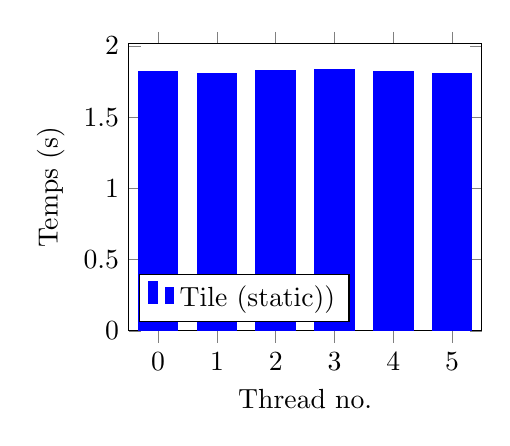
\begin{tikzpicture}
\begin{axis}[
  ybar,
  bar width=0.5cm,
  xlabel={Thread no.},
  ylabel={Temps (s)},
  ymin=0,
  legend pos=south west,
  width=0.5\textwidth,
  xtick=data
]

% Données pour le premier graphique (à gauche)
\addplot[color=blue, fill=blue] coordinates {
  (0,1.822252) (1,1.808600) (2,1.823853) (3,1.831479) (4,1.819218) (5,1.805120)
};
\addlegendentry{Tile (static))}

\end{axis}
\end{tikzpicture}
\hfill
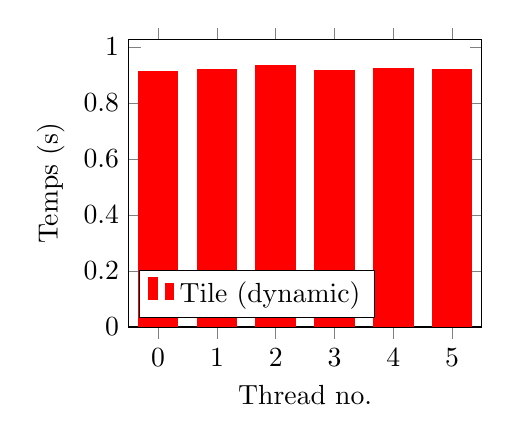
\begin{tikzpicture}
\begin{axis}[
  ybar,
  bar width=0.5cm,
  xlabel={Thread no.},
  ylabel={Temps (s)},
  ymin=0,
  legend pos=south west,
  width=0.5\textwidth,
  xtick=data
]

% Données pour le deuxième graphique (au milieu)
\addplot[color=red, fill=red] coordinates {
  (0,0.913124) (1,0.919698) (2,0.932781) (3,0.914996) (4,0.924028) (5,0.921380)
};
\addlegendentry{Tile (dynamic)}

\end{axis}
\end{tikzpicture}
\hfill
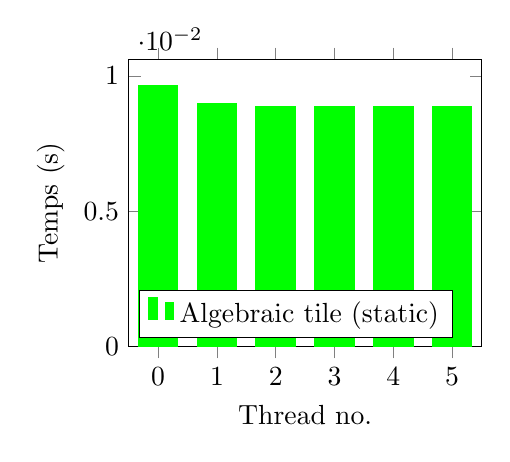
\begin{tikzpicture}
\begin{axis}[
  ybar,
  bar width=0.5cm,
  xlabel={Thread no.},
  ylabel={Temps (s)},
  ymin=0,
  legend pos=south west,
  width=0.5\textwidth,
  xtick=data
]

% Données pour le troisième graphique (à droite)
\addplot[color=green, fill=green] coordinates {
  (0,0.009643) (1,0.008962) (2,0.008869) (3,0.008870) (4,0.008864) (5,0.008867)
};
\addlegendentry{Algebraic tile (static)}

\end{axis}
\end{tikzpicture}

\caption{Temps d'exécution des threads pour le fichier gramschmidt.c}
\label{fig:graphes}
\end{figure}

\begin{table}[htbp]
  \centering
  \caption{Statistiques pour le fichier gramschmidt.c}
  \begin{tabular}{|c|c|c|c|}
    \hline
    Statistique & Algebraic Tile & Tile (static) & Tile (dynamic) \\ 
    \hline
    Skewness (g1) & 1.73252 & -0.19406 & 0.599313 \\ 
    Kurtosis (g2) & 1.08975 & -1.22229 & -0.608269 \\ 
    Écart type & 0.000284078 & 0.00902495 & 0.00642754\\ 
    Percent Imbalance metric en \% & 6.99584 & 0.718151 & 1.27904\\ 
    Temps moyen (s) & 0.009643 & 1.831479 & 0.932781 \\ 
    \hline
  \end{tabular}
\end{table}
\newpage

  \end{document}
